\section{Développement Technique}

\subsection{Gestion des erreurs}
\label{sec:error_handling}

Pour gérer les erreurs dans notre application, nous avons utilisé \texttt{either}, qui permet de retourner une erreur si une opération n'a pas fonctionné, et de renvoyer les données si elle a réussi. De cette manière, nous pouvons gérer facilement l'erreur au front-end. Ensuite, nous avons créé des classes avec des exceptions et des erreurs spécifiques pour pouvoir les afficher à l'utilisateur. Il est essentiel que ces erreurs soient bienveillantes et compréhensibles pour l'utilisateur, et qu'elles ne soient pas techniques. Ainsi, l'utilisateur peut facilement comprendre ce qui s'est passé et comment rectifier la situation, sans être inquiété par des messages d'erreur trop complexes ou techniques.


\subsection{Peuplement de la base de données}

Pour peupler la base de données de notre application, nous avons rassemblé des données disponibles librement et publiquement sur Internet, en particulier sur les sites de la Migros, de la Coop et de Denner. Ces sites fournissent des métadonnées des articles, incluant leurs prix et des images associées. Nous avons débuté par la création d'un script en Dart qui intègre les produits, certaines métadonnées, ainsi que quelques types de produits et utilisateurs, afin de tester l'application de manière adéquate. Ce script se connecte à Firestore et envoie les données sur Firebase, ce qui permet de peupler efficacement la base de données. Bien que ce script manuel soit initialement utilisé pour insérer les données nécessaires au test de l'application, nous envisageons à l'avenir de développer un scraper web. Ce scraper pourrait automatiser la récupération des données de tous les produits des sites de la Migros, de la Coop, etc., garantissant ainsi une base de données complète et constamment mise à jour. Grâce à cette automatisation, nous pourrions maintenir une base de données riche et précise, essentielle pour le bon fonctionnement de l'application.

\subsection{Internationalisation}
\label{sec:i18n}

Nous avons localisé notre application avec le mécanisme d'internationalisation (i18n) de Flutter. Concrètement, nous avons créé un fichier utilitaire i18n qui nous permet de gérer les différentes traductions de l'application. Chaque langue est représentée par un fichier de traduction spécifique, dans lequel sont stockées les chaînes de caractères traduites. Le processus de traduction commence par l'identification des chaînes de texte à traduire dans l'application. Ensuite, ces chaînes sont externalisées dans les fichiers de traduction, où chaque langue dispose de ses propres traductions. Grâce à ce système, l'application peut automatiquement afficher le texte dans la langue choisie par l'utilisateur, en fonction des paramètres de son appareil. Bie que nous n'ayons pas eu le temps de traduire toutes les chaînes de texte de l'application, le principe de l'internationalisation est entièrement implémenté et fonctionnel. Ainsi, l'ajout de nouvelles traductions peut se faire rapidement et efficacement à mesure que de nouvelles langues sont prises en charge ou que de nouvelles chaînes de texte sont ajoutées à l'application.

\subsection{Modélisation des Données}
\label{sec:data_model}

La structure de données d'EthiScan, illustrée dans la figure \ref{fig:diagramme_classe} a été conçue pour permettre une gestion efficace et évolutive des informations produits et des préférences utilisateurs.

La classe principale \texttt{EthiscanUser} représente un utilisateur de l'application, incluant ses produits favoris (\texttt{FavoriteProduct}), ses préférences (\texttt{UserPreferences}), et un Firebase \texttt{User} contenant des informations d'authentification comme l'identifiant, le nom et l'email. Chaque \texttt{FavoriteProduct} référence un \texttt{Product} avec une date d'ajout, permettant à l'utilisateur de suivre ses produits préférés.

La classe \texttt{Product} représente les produits scannés par les utilisateurs. Chaque produit peut avoir une certification (\texttt{Certification}) et est associé à une liste de métadonnées spécifiques (\texttt{ProductMetadata}). Cette séparation entre le type de métadonnées (\texttt{MetadataType}) et les instances spécifiques des métadonnées permet une gestion flexible des différentes informations que les utilisateurs peuvent consulter.

Les fournisseurs (\texttt{Supplier}) sont modélisés pour contenir une liste de produits vendus (\texttt{SoldProduct}), chacun ayant un prix spécifique. Cette approche permet de gérer les variations de prix d'un même produit chez différents fournisseurs.

Enfin, les préférences utilisateur (\texttt{UserPreferences}) sont représentées par une liste de types de métadonnées auxquels l'utilisateur est abonné. Ces abonnements permettent à l'utilisateur de recevoir des informations personnalisées et pertinentes en fonction de ses valeurs et de ses préférences de consommation.

\begin{figure}[h]
    \centering
    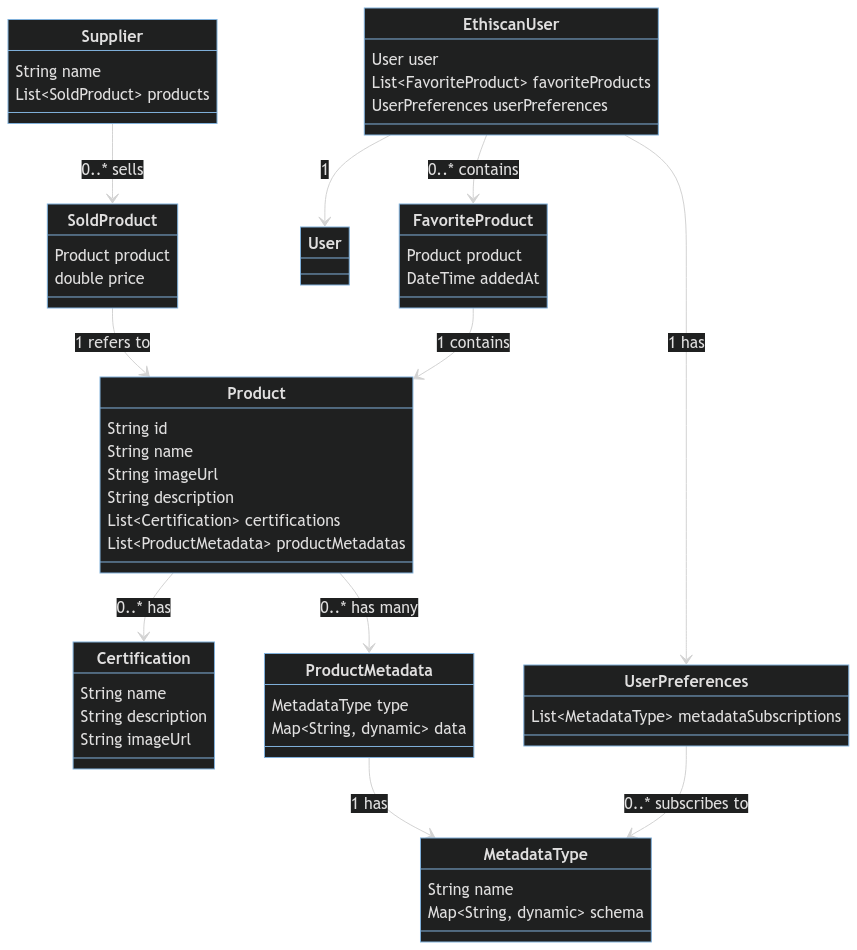
\includegraphics[width=0.6\textwidth]{/home/olivier/projet/advanced_mobile_app/concept/rapport/images/diagramme_classe.png}
    \caption{Diagramme de classe de l'application}
    \label{fig:diagramme_classe}
\end{figure}

\subsection{Intégration Continue et Déploiement Continu (CI/CD)}
\label{sec:ci_cd}
Pour automatiser le processus de développement et de déploiement de notre application mobile, nous avons mis en place des GitHub Actions. Ces workflows permettent de s'assurer que chaque modification apportée au code est correctement testée et que les versions de l'application sont déployées de manière fluide. Nous avons segmenté notre approche CI/CD en deux parties distinctes : l'intégration continue (CI) et le déploiement continu (CD).

\subsubsection{Intégration Continue (CI)}

L'intégration continue est déclenchée à chaque fois qu'un commit est effectué dans le dépôt GitHub. Le but principal de la CI est de garantir la qualité et la cohérence du codebase. Pour ce faire, nous avons configuré GitHub Actions pour exécuter les tests unitaires et le linter sur l'ensemble du code. En particulier, nous utilisons la commande \texttt{flutter analyze} pour analyser notre code Flutter. Cette analyse permet de détecter les erreurs et les incohérences dans le code, facilitant ainsi la collaboration entre les développeurs et assurant que le code est toujours dans un état prêt à être fusionné.

\subsubsection{Déploiement Continu (CD)}

Le déploiement continu est activé à chaque fois qu'un tag est poussé sur le dépôt. Ce processus comprend la construction de l'application et son déploiement. Nous avons configuré une action pour compiler l'application et générer les fichiers APK nécessaires. Une fois la construction terminée, les fichiers APK sont automatiquement envoyés sur notre groupe Telegram. Ceci permet à l'équipe de disposer immédiatement des nouvelles versions de l'application.

\subsection{Problèmes Rencontrés et Solutions}
\label{sec:problems}

\paragraph{Version des dépendances} Lors du développement, nous avons rencontré un problème majeur lié à la gestion des versions de Flutter utilisées par les différents membres de l'équipe. En effet, nous avons constaté qu'une personne utilisait la version 3.22 de Flutter, tandis que d'autres travaillaient avec la version 3.19. Cette disparité de versions a causé des conflits lors de l'intégration de nouvelles dépendances. Par exemple, certaines dépendances étaient compatibles avec une version de Flutter mais pas avec l'autre, ce qui a entraîné des erreurs de compilation. La synchronisation des versions de Flutter entre tous les membres de l'équipe s'est avérée difficile. Nous avions le choix entre downgrade Flutter ou de résoudre les conflits avec la dernière version. Nous avons opté pour la deuxième option, car elle nous permettait de bénéficier des dernières fonctionnalités et correctifs de Flutter. Cependant, cela a nécessité un effort supplémentaire pour résoudre les conflits et garantir la compatibilité des dépendances avec la version la plus récente de Flutter. Des bugs qui se sont avéré très chronophage ont aussi été rencontré avec nos outils de développement. Un membre de notre équipe a notamment eu des problèmes de dépendances qui n'a pu être résolut qu'en redémarrant VS-Code.

\paragraph{Structure de l'application} Nous avons décidé de suivre les bonnes pratiques de la "clean architecture" ce qui a posé plusieurs défis. Comme chaque membre de l'équipe avait une expérience différente Flutter, nous avons tous développé des portions de code de manière indépendante, en utilisant des approches et des structures différentes, souvent inspirées d'exemples trouvés en ligne ou de projets précédents. L'intégration de ces morceaux de code disparates dans un cadre uniforme basé sur la clean architecture a nécessité des efforts significatifs. Nous avons dû refactorer et harmoniser les différentes méthodes de développement pour les aligner avec les principes de la clean architecture, ce qui a parfois causé des problèmes d'intégration et ralenti le développement de nouvelles features. Cette étape a souligné l'importance de définir dès le départ une architecture claire et partagée par toute l'équipe pour faciliter le développement collaboratif. Au final, nous avons utilisé le package "clean\_architecture" pour structurer notre application.

\paragraph{Gestion des états} Un autre défi a été la gestion des blocs, en particulier avec les pages de connexion et d'inscription. Initialement, nous avions un mainUserBloc chargé de l'authentification et de la gestion des données utilisateur dans toute l'application. Cependant, l'intégration des pages de connexion et d'inscription a posé problème. Ces pages, conçues pour fonctionner indépendamment, ne s'intégraient pas bien dans la structure de l'application en raison de problèmes liés aux locales de traduction. Pour contourner ce problème, nous avons décidé de placer ces pages directement dans le fichier app.dart, en dehors de la structure principale de l'application. Cette décision a introduit des complications avec le main user bloc, entraînant des conflits entre les blocs de gestion d'état. Bien que nous ayons finalement trouvé une solution. TODO Quelle solution ? Comment on a fix ce truc ?
%fix todo above
\paragraph{Versionnement du code} Nous avons rencontré quelques problèmes avec l'utilisation de GitHub au sein de notre équipe. L'un des membres, ne maîtrisant pas GitHub, a effectué tout son travail sur une branche existante déjà mergée sur la principale (main), sans jamais fusionner ses modifications. Par conséquent, le reste de l'équipe n'a pas pu suivre l'avancement de son travail. Au moment de fusionner sa branche, nous avons découvert le problème. Cela a posé des problèmes d'intégration car le code sur main avait été largement restructuré entre-temps. Pour résoudre cette situation, nous avons résolu les conflits de versions progressivement jusqu'au succès. Puis, nous avons formé toute l'équipe à l'utilisation de GitHub. Désormais, chaque nouvelle tâche doit être accompagnée de la création d'une issue et d'une branche correspondante. Une fois la tâche terminée et approuvée, la branche est fusionnée dans la branche principale avec un code review. Cette approche, combinée à une meilleure communication entre les membres de l'équipe, a permis d'éviter les problèmes.

\paragraph{Déploiement Continu} Le déploiement a posé quelques difficultés, principalement liées à la gestion sécurisée du fichier \texttt{google-service.json}, indispensable pour la construction et le déploiement de l'application sur notre groupe Telegram. Comme ce fichier contient des informations sensibles, nous devons le sécuriser et le stocker dans un endroit accessible par notre pipeline CI/CD. Pour résoudre ce problème, nous avons décidé de stocker \texttt{google-service.json} en tant que action secret dans GitHub. Cependant, un problème de formatage est apparu lors de la gestion de ce secret. Pour le surmonter, nous avons encodé le fichier en base64 avant de le stocker dans GitHub Secrets. Ce qui a résolu le problème de formatage et nous a permis de déployer l'application avec succès de manière sécurisée.

\paragraph{Développement Automatisé}
Pour accélérer le développement, nous avons intégré le package \texttt{Freezed} et encore le package \texttt{json\_encode}, destiné à compiler et générer automatiquement certaines parties du code. Cette automatisation vise à réduire le code répétitif, augmentant ainsi notre productivité et permettant de se concentrer sur des aspects plus critiques du développement. Cependant, l'introduction de ce package a posé des défis pour un membre de l'équipe non familier avec cette technologie. En effet, il rencontrait des difficultés à déboguer son code, n'ayant pas une maîtrise complète des processus automatisés par \texttt{Freezed}. Ce manque de compréhension a entraîné des erreurs de compilation et une perte de temps significative pour cette personne, contrebalançant ainsi les bénéfices attendus de l'automatisation. Pour résoudre ce problème, nous avons organisé une session de discussion afin de clarifier l'utilisation du script \texttt{Freezed} et de bien séparer les concepts. Après cette mise au point, il n'a plus rencontré de problèmes de compilation, et l'équipe a pu bénéficier pleinement des gains de productivité promis par l'automatisation. Cette expérience souligne l'importance de l'accompagnement et de la formation lors de l'intégration de nouvelles technologies dans un projet de développement.


\subsection{Conclusion Technique}

La combinaison de Flutter et Firebase a prouvé son efficacité pour développer une application mobile performante et réactive. L'architecture choisie a permis une mise en œuvre rapide des fonctionnalités tout en maintenant une haute qualité et fiabilité des données.

\section{Auto-Critique du Code}

\subsection{Points Positifs}

\paragraph{Flexibilité}
L'implémentation partielle de la clean architecture dans notre application nous offre une flexibilité en termes de gestion des providers de données. Par exemple, si nous décidons de remplacer \texttt{Firebase} par \texttt{Supabase} par exemple, il suffit de réimplémenter les datasources sans modifier le reste de l'application. Cette modularité nous rend résilients face aux évolutions technologiques et aux changements de fournisseurs de services, assurant ainsi la pérennité de notre application.

\paragraph{Modélisation robuste des données}
Notre application bénéficie d'une modélisation des données bien structurée et robuste. Cette modélisation permet non seulement de gérer efficacement les données actuelles, mais aussi de faire évoluer le système pour accueillir plusieurs centaines de milliers d'utilisateurs si nécessaire. Grâce à cette architecture scalable, notre application est prête à grandir et à s'adapter aux besoins croissants des utilisateurs, garantissant une performance et une fiabilité optimales à long terme.

\paragraph{Pratiques de développement logiciel}
Nous avons implémenté de nombreuses pratiques de développement logiciel qui ont grandement facilité notre travail. L'intégration continue (CI) et le déploiement continu (CD) nous permettent d'automatiser les processus de test et de déploiement, assurant une détection rapide des erreurs et des mises à jour fluides de l'application. L'internationalisation a été intégrée pour rendre notre application accessible à un public mondial. De plus, en utilisant la clean architecture, nous avons structuré notre code de manière modulaire et maintenable. L'utilisation de GitHub pour la gestion de version, avec des branches et des pull requests, a amélioré notre collaboration et notre efficacité. Toutes ces pratiques combinées a augmenté notre productivité et nous a aidé à maintenir une haute qualité de code.





\subsection{Points à Améliorer}

Pour améliorer le développement de notre application mobile, nous avons identifié plusieurs aspects nécessitant des améliorations.

\paragraph{Augmentation de la couverture des tests unitaires}
Actuellement, la couverture de code par nos tests unitaires est insuffisante. Les tests unitaires sont très limités et ne couvrent pas l'ensemble des fonctionnalités critiques de l'application. Pour garantir une meilleure qualité et fiabilité du code, il est impératif d'augmenter la couverture des tests unitaires. Cela inclut l'ajout de tests pour les cas limites, les scénarios d'erreur, ainsi que les interactions complexes entre les différents composants de l'application.

\paragraph{Renforcement de la sécurité des données}
Pour des raisons de développement, les règles de sécurité de notre base de données Firestore sont actuellement complètement ouvertes. Cette configuration est inadmissible dans un environnement de production réel. Il est crucial de mettre en place des règles de sécurité strictes afin de gérer correctement les autorisations des utilisateurs. Chaque utilisateur doit uniquement pouvoir accéder et modifier ses propres données. Par exemple, les règles de sécurité doivent garantir qu'un utilisateur ne puisse pas supprimer ou accéder aux produits favoris d'un autre utilisateur. Le renforcement de ces mesures de sécurité est impératif pour la mise en production de l'application.

\paragraph{Amélioration de la clean architecture}
Actuellement, notre implémentation de la clean architecture est partielle. Les blocs gèrent directement les use cases, ce qui va à l'encontre des principes de séparation des préoccupations et rend les blocs plus difficiles à tester et complexes à maintenir. Pour se rapprocher davantage de la clean architecture, il serait judicieux de séparer les use cases des blocs. Les use cases doivent être implémentés de manière indépendante et injectés dans les blocs, ce qui facilitera les tests unitaires et simplifiera le code.

